\section{Methodology}\label{sec:Methodology}
The Tsception model has a convolutional architecture. It majorly consists of 3 important layers- The dynamic temporal layer, spatial assymmetric layer and high level fusion layer.The input to the model is the raw EEG signal consisiting of various temporal and spatial features. This raw EEG signal is passed to the Temporal layer which has several multiscale convolutional kernels. These help in capturing the finer temporal dependencies. The output of this temporal layer is passed to the spatial assymmetric layer where the spatial features are learnt. The high level fusion layer fuses the outputs giving a high level representation of the data which is then fed to the fully connected network which in turn maps it to its corresponding labels.
\subsection*{Dynamic Temporal Layer}
The dynamic temporal layer is designed to unravel the intricate temporal patterns embedded in the EEG signals. The kernels are structured to capture temporal patterns at different scales. These kernel sizes are determined by the sampling rates of the EEG signals. These ratios are specified by $\alpha$, which in our model takes the values $0.125$, $0.25$, $0.5$. The input EEG samples are processed through these kernels. For each level, a 1D convolution operation applies the corresponding kernel to the input. This operation helps in extracting features from the EEG signals that correspond to different temporal and frequency characteristics based on the kernel size. Post convolution, the feature map is passed through the Leaky-ReLU activation function, which introduces non-linearity in the model enabling it to learn complex patterns. This EEG output is further downsampled via average pooling. The output of $i$-th convolution sample is 
\[
Z_i^{\text{temporal}} = \text{AP} \left( \Phi_L^{\text{ReLU}} \left( \text{Conv1D}(X, s_i^T) \right) \right)
\]
Each level of the dynamic temporal layer produces a temporal feature map. These maps from different levels are then concatenated along the feature dimension. This concatenation captures all the temporal features across all the scales, enriching the representation of the EEG signals. A standard batch normalization is applied to this cocatenated output to ensure that the model is robust to the changes in the input distribution.
\begin{figure*}[htbp]
    \centering
    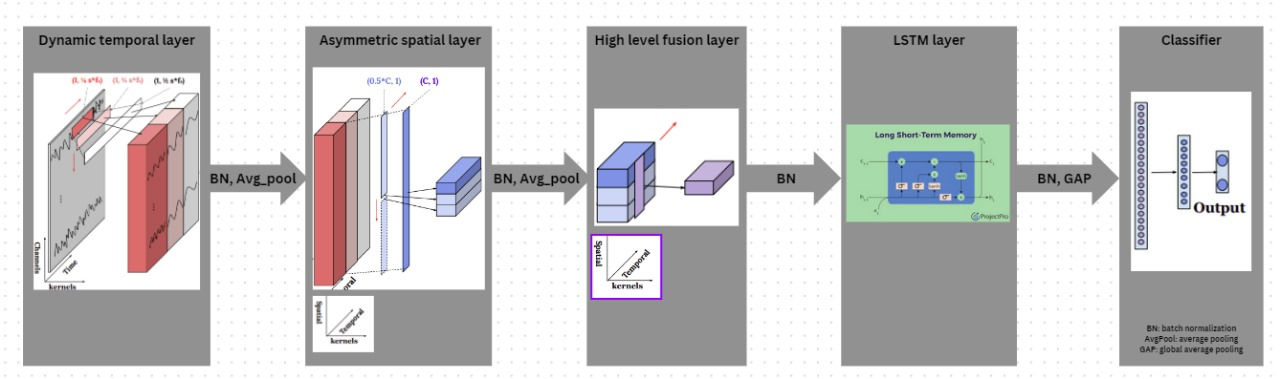
\includegraphics[width=\textwidth]{diagram.jpeg}
    \caption{New model architecture}
    \label{fig:yourlabel}
  \end{figure*}

\subsection*{Spatial Assymmetric Layer}
The assymmetric spatial layer is designed to capture the spatial patterns reflecting structural and functional assymetry of the human brain. It particularly focuses on differences between left and right hemispheres.It uses multi scale  $1$ D convolutional kernels to analyze the data. These patterns are aptly captured the spatial arrangement of the EEG channels on the scalp.
\subsubsection*{Types of Spatial Kernels}

\begin{itemize}
    \item \textbf{Global Kernel:} This kernel has a size of \((c, 1)\), where \(c\) is the total number of channels. It spans all channels at a time enabling it to capture global spatial information from the entire array of EEG channels.
    \item \textbf{Hemisphere Kernel:} This kernel, size \((0.5 \cdot c, 1)\) with a stride of \((0.5 \cdot c, 1)\), specifically targets the relationships between the left and right hemispheres. The kernel is shared between corresponding locations on each hemisphere, facilitating the extraction of asymmetrical patterns without overlapping.
\end{itemize}
After convolution with the global kernel, the output feature map is given by:
\begin{align*}
    \text{Output feature map} &\Rightarrow \dim(n, 1, f)
\end{align*}

After convolution with each hemisphere kernel:
\begin{align*}
    \text{1\textsuperscript{st} half: feature map} &\Rightarrow \dim(n, 1, f) \\
    \text{2\textsuperscript{nd} half: feature map} &\Rightarrow \dim(n, 1 , f)
\end{align*}

Concatenating the two halves yields:
\begin{align*}
    \text{Concatenated feature map} &\Rightarrow \dim(n, 3, f)
\end{align*}

Both the kernels apply $1$ D convolution operation to the output of the dynamic temporal layer. After convolution, feature maps are passed through the Leaky-Relu to introduce non linearity followed by average pooling and batch normalisation.

\subsection*{High Level Fusion Layer}
This layer integrates the spatial information extracted from the Assymmetric spatial layer from global and hemisphere kernels. It is is $1$ D convolutional layer with kernel size $(3, 1)$. Subsequently, Leaky-Relu,average pooling layer, batch normalisation and GAP layer are applied on the convolutional output.

This gives a high level representation of the data which is fed to the fully connected network fro training which can learn complex relationships between the fused features.To produce probability distribution over the target classes,a softmax fucntion is used.

\subsection*{LSTM Layer}
The input to the LSTM layer is the output of the fusion layer which is batch normalised. The mean is computed along the last dimension, preparing the data to have suitable shape to pass through LSTM.The LSTM structure is defined with a specified number of input features \((\text{num\_S})\), a hidden state size \((\text{lstm\_hidden})\), and it is set to have the batch data first \((\text{batch\_first} = \text{True})\). This configuration is crucial as it dictates how the LSTM processes the input data and the dimensionality of the output.
The LSTM processes the input sequence in a recurrent fashion, updating its hidden states and cell states at each time step.
It provides two outputs the hidden states for all time steps and the cell states. For our classification the last hidden state is used for the final classification.
The \texttt{fc\_lstm} is a sequence of fully connected layers (linear layers in PyTorch) with a ReLU activation and dropout for regularization. The final layer maps the hidden state to the number of classes for classification.

% \begin{figure}[h]
%     \centering
%     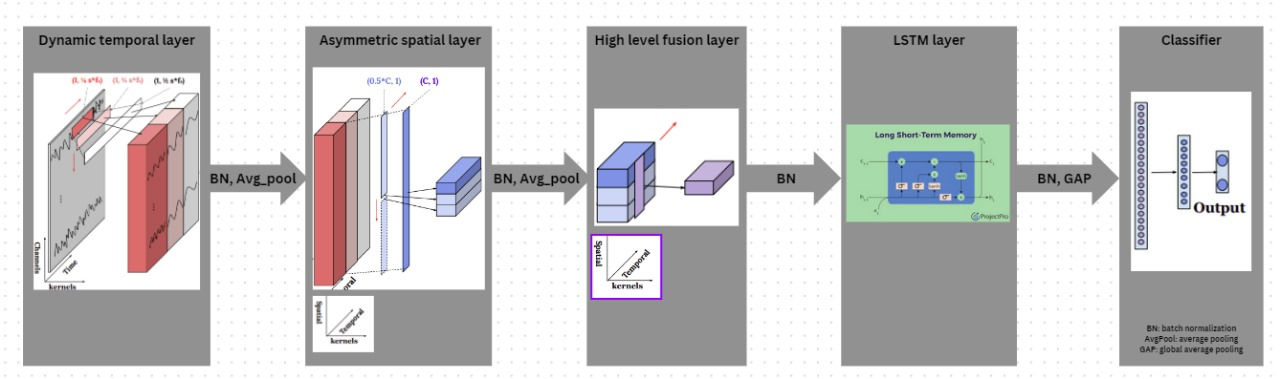
\includegraphics[width=0.5\textwidth]{diagram.jpeg} % Adjust the path and the scaling factor
%     \caption{New model architecture} % Caption for the image
%     \label{New model architecture} % Label for referencing the image elsewhere in the text
% \end{figure}

  
